\documentclass[lang=cn,11pt,a4paper,cite=authornum]{paper}

\title{形式语言与自动机实验二:设计上下文无关文法的变换算法\ 实验报告}
\author{毛子恒 \and 邹宇江 \and 王敏行 \and 曾嘉伟}
\institute{北京邮电大学\ 计算机学院}

\date{\zhtoday}

% 本文档命令
\usepackage{array}
\newcommand{\ccr}[1]{\makecell{{\color{#1}\rule{1cm}{1cm}}}}
\nocite{*}

\begin{document}

\maketitle

\section*{小组成员}

\setlength{\tabcolsep}{7mm}
{
    \begin{table}[htbp]
        \centering
        \begin{tabular}{llll}
            班级:2019211309 & 姓名:毛子恒 & 学号:2019211397 & 分工:代码\ 文档 \\

            班级:2019211309 & 姓名:邹宇江 & 学号:2019211416 & 分工:测试\ 文档 \\

            班级:2019211309 & 姓名:王敏行 & 学号:2019211410 & 分工:测试\ 文档 \\

            班级:2019211309 & 姓名:曾嘉伟 & 学号:2019211396 & 分工:测试\ 文档 \\
        \end{tabular}
    \end{table}
}

\section{需求分析}

\subsection{题目描述}

编程实现上下文无关文法的变换算法,用于消除文法中的$\varepsilon$产生式、单产生式以及无用符号。

\subsection{输入描述}

程序从标准输入中读入数据。

以下描述中\textbf{字符串}均特指不包含空格、回车等特殊字符的ASCII字符序列。\textbf{要求输入是一个合法的上下文无关文法}。

第一行输入若干字符串,用空格分隔,表示上下文无关文法$\mathbf G$的非终止符集合$\mathbf N$,\textbf{要求输入不出现重复符号}。

第二行输入若干字符串,用空格分隔,表示上下文无关文法$\mathbf G$的终止符集合$\mathbf T$,\textbf{要求输入不出现重复符号}。

接下来的若干行,表示上下文无关文法$\mathbf G$的生成式集合$\mathbf P$。每行若干个字符串,其中第一个字符串表示生成式左边的符号,其余字符串依次为生成式右边的符号,\textbf{要求输入的符号均包含在$\mathbf N \cup \mathbf T$中}。使用特殊的字符串"[empty]"表示空串。以一个空行表示$\mathbf P$的结束。

最后一行输入一个字符串,表示起始符,\textbf{要求起始符包含在$\mathbf N$中}。

\subsection{输出描述}

程序向标准输出中输出提示信息和每一步算法的运行结果。

\subsection{样例}

\subsubsection{样例输入}

\begin{code}
\begin{minted}[frame=lines]{bash}
S A B C D
a b c d
S a
S b A
S B
S c c D
A a b B
A [empty]
B a A
C d d C
D d d d

S
\end{minted}
\end{code}

\subsubsection{样例输出}

\begin{code}
\begin{minted}[frame=lines]{bash}
N: {S, B, D, A, C, }
T: {c, b, d, a, }
P:
        S -> a | B | bA | ccD | 
        A -> abB | [empty] | 
        B -> aA | 
        C -> ddC | 
        D -> ddd | 
S: S
消去epsilon产生式
N: {S, B, D, A, C, }
T: {c, b, d, a, }
P:
        S -> ccD | a | b | B | bA | 
        A -> abB | 
        B -> a | aA | 
        C -> ddC | 
        D -> ddd | 
S: S
消去单产生式
N: {S, B, D, A, C, }
T: {c, b, d, a, }
P:
        S -> ccD | aA | a | b | bA | 
        B -> a | aA | 
        D -> ddd | 
        A -> abB | 
        C -> ddC | 
S: S
消去无用符号
N: {A, D, S, B, }
T: {a, c, b, d, }
P:
        S -> ccD | aA | a | b | bA | 
        B -> a | aA | 
        D -> ddd | 
        A -> abB | 
S: S
\end{minted}
\end{code}

\subsubsection{样例运行结果}

见\figref{fig:result}。

\begin{figure}[htbp]

    \centering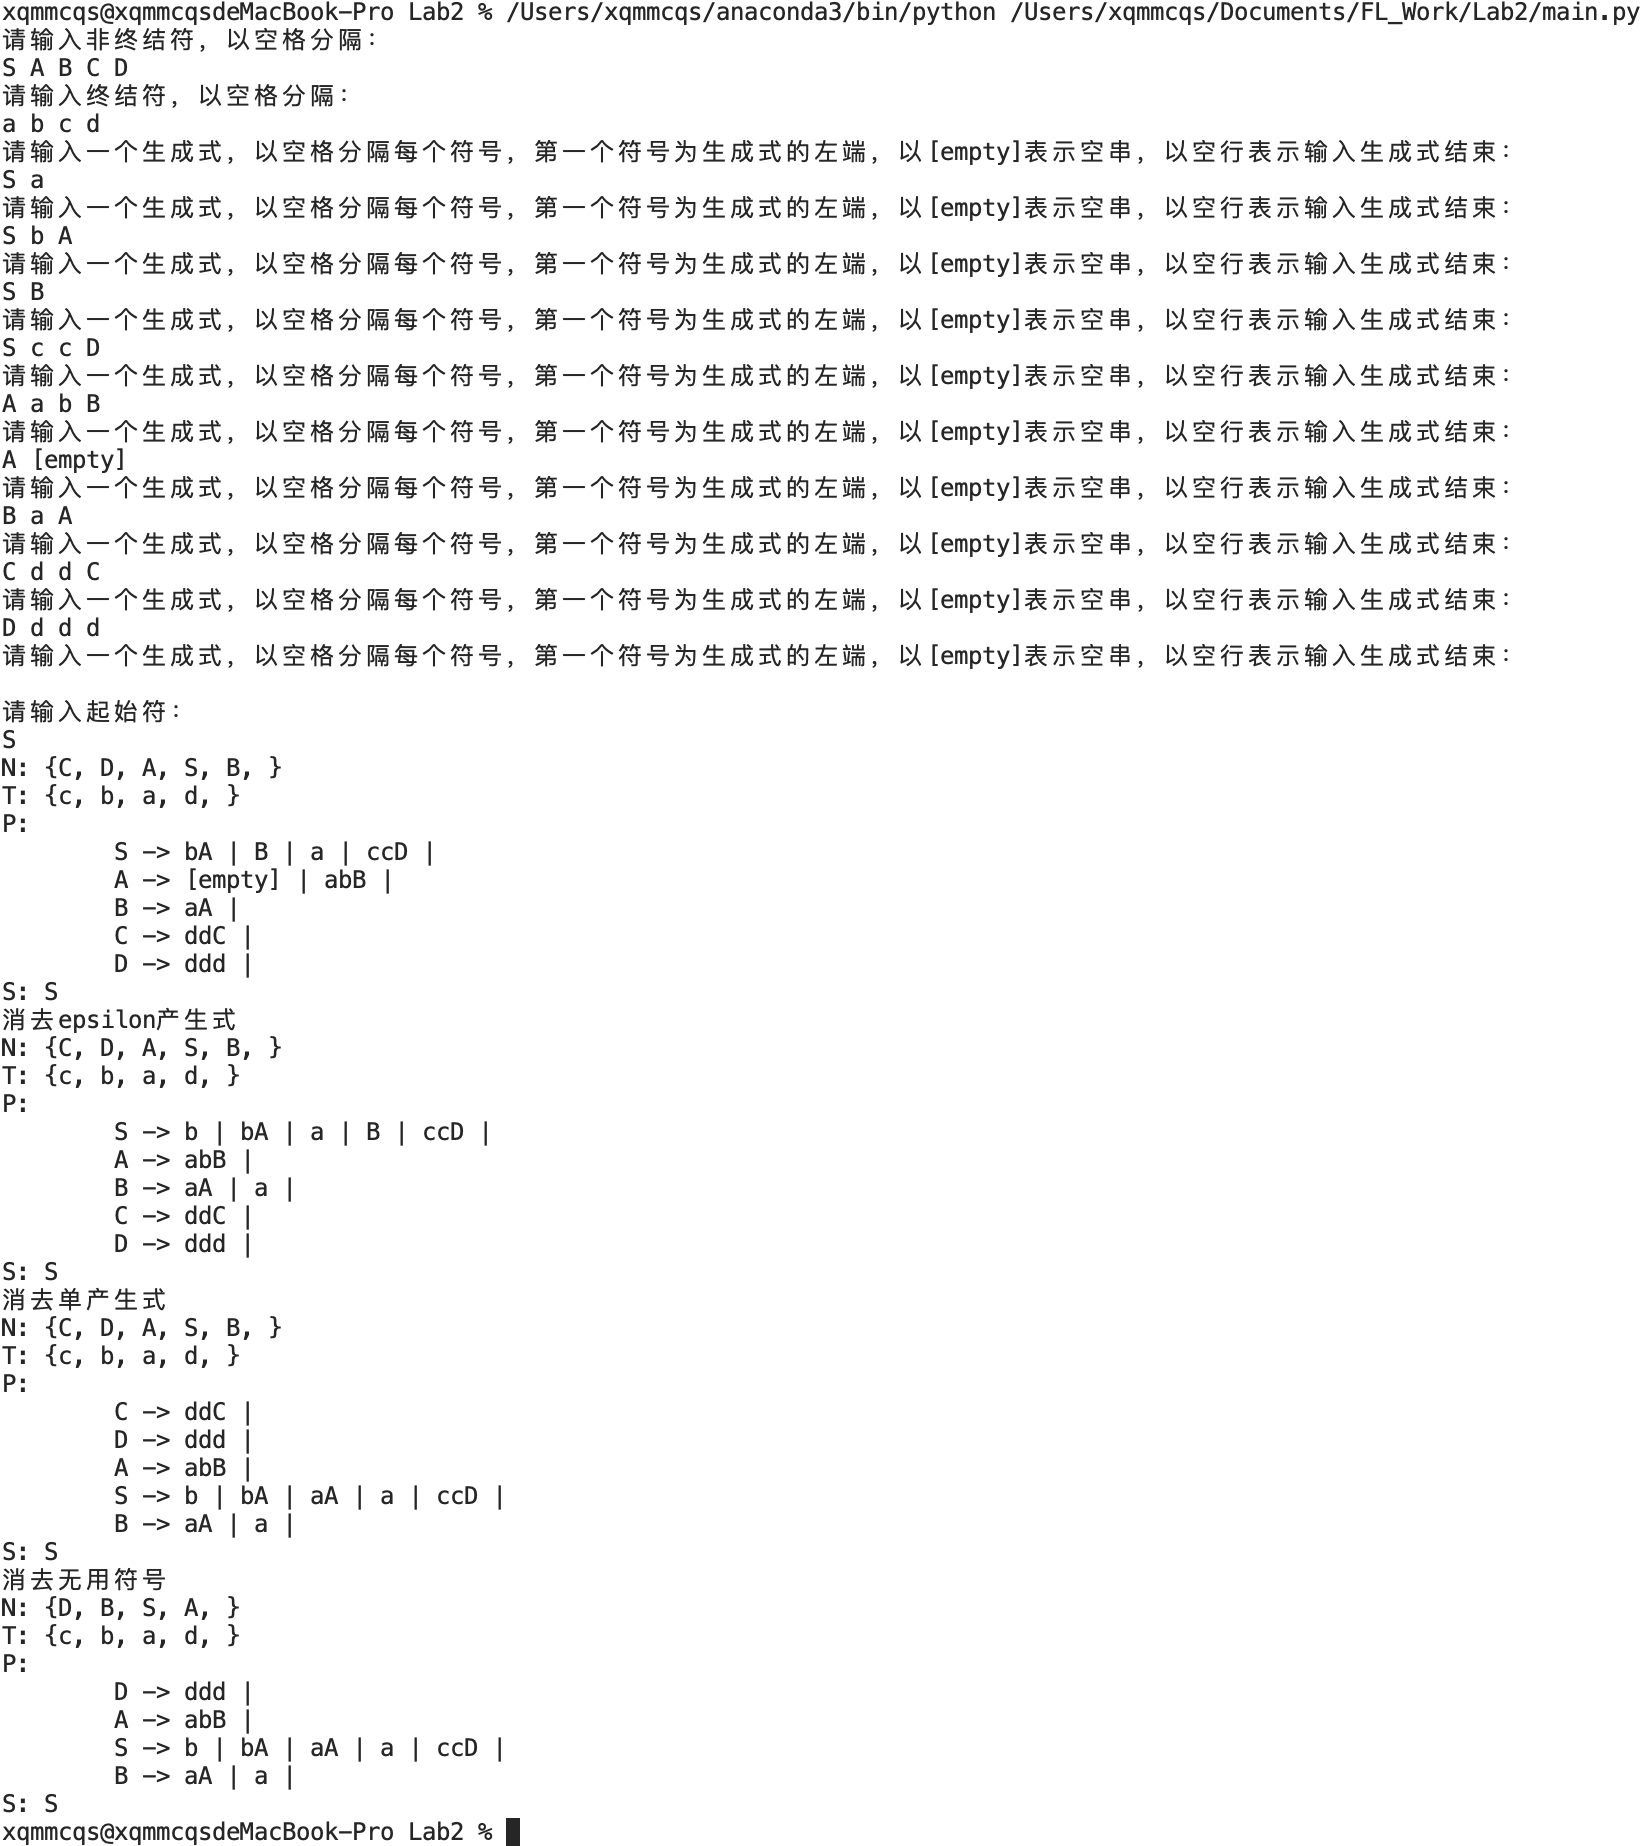
\includegraphics[width=\textwidth]{./Images/result.png}

    \caption{样例运行结果\label{fig:result}}

\end{figure}

\section{程序设计}

\subsection{环境}

\begin{itemize}
    \item macOS Big Sur 11.3
    \item Python 3.7.9
\end{itemize}

\subsection{设计思路}

将符号用字符串表示,$\mathbf G$和$\mathbf T$用Python集合表示,$\mathbf P$用Python字典表示,字典的键为生成式左端的符号,值为一个列表,列表的元素是元组,元组内的每个元素是一个符号。

例如,$S\rightarrow a|bA|ccD$表示成字典中的一个元素是:\mintinline{Python}{{'S': [('a',), ('b', 'A'), ('c', 'c', 'D')]}}

在消去$\varepsilon$产生式的算法中,涉及到将$Y_i$取$C_i$或$\varepsilon$的所有组合枚举出来(共$2^n$种),我采用枚举二进制数的方法,枚举$num\in[0,2^n-1]$,如果$num$的第$i$位是1,则$Y_i=C_i$,否则$Y_i=\varepsilon$。

判断$\omega\in \mathbf N^*$时,需要判断$\forall a\in\omega, a\in\mathbf N$,枚举$\mathbf P$需要二重循环,除此之外所有的操作基本都是集合与元素的操作,和伪代码几乎完全一致。

\subsection{核心算法伪代码}

消去$\varepsilon$产生式的伪代码见\algoref{algo:eliepsi};消去单产生式的伪代码见\algoref{algo:elising};消去无用符号的伪代码见\algoref{algo:eliusel};

\begin{algorithm}[htbp]
    \caption{消去$\varepsilon$产生式\label{algo:eliepsi}}
    \KwIn{$\mathbf G = (\mathbf N, \mathbf T, \mathbf P, S)$}
    \KwOut{$\mathbf G_1 = (\mathbf N_1, \mathbf T, \mathbf P_1, S_1)$}
    \SetKwProg{Fn}{Function}{}{end}
    \SetKwData{Nz}{$\mathbf {N_0}$}
    \SetKwData{Np}{$\mathbf {N'}$}
    \SetKwData{P}{$\mathbf P$}
    \SetKwData{Po}{$\mathbf P_1$}
    \SetKwData{Tot}{total}
    \SetKwData{Num}{num}
    \SetKwFunction{EliEpsi}{eliminate\_epsilon}
    \Fn(){\EliEpsi{}}{
        $\Nz\leftarrow \varnothing$\;
        $\Np\leftarrow \varnothing$\;
        \ForEach{$A\rightarrow \varepsilon \in \P$}{
            $\Np \leftarrow\Np \cup \{A\}$\;
        }
        \While{$\Nz \not= \Np$}{
            $\Nz \leftarrow \Np$\;
            \ForEach{$A\rightarrow \omega \in \P$}{
                \lIf{$\omega\in\mathbf N_0^*$}{$\Np \leftarrow\Np \cup \{A\}$}
            }
        }
        $\Po\leftarrow\varnothing$\;
        \ForEach{$A\rightarrow \omega\in\P$}{
            $n\leftarrow |\{C|C\in \omega\wedge C\in \Np\}|$\;
            \For{$\Num\leftarrow 0$ \KwTo $2^n-1$}{
                \tcp{$\Num = \sum_{i=0}^n \Num_i\times 2^i$}
                $\omega_1\leftarrow\varepsilon$\;
                \Tot$ \leftarrow 0$\;
                \ForEach{$a\in\omega$}{
                    \If{$a\in\Np$}{
                        \lIf{$\Num_{\Tot}=1$}{$\omega_1\leftarrow\omega_1 a$}
                        \Tot$\leftarrow$\Tot$+1$\;
                    }
                    \lElse{$\omega_1\leftarrow\omega_1a$}
                }
                \lIf{$\omega_1\not=\varepsilon$}{$\Po\leftarrow\Po\cup\{A\rightarrow \omega_1\}$}
            }
        }
        \If{$S\in\Np$}{
            $\Po\leftarrow\Po\cup\{S_1\rightarrow\varepsilon, S_1\rightarrow S\}$\;
            $\mathbf N_1\leftarrow\mathbf N\cup \{S_1\}$\;
        }
        \Else{
            $\mathbf N_1\leftarrow\mathbf N$\;
            $S_1\leftarrow S$\;
        }
    }
\end{algorithm}

\begin{algorithm}[htbp]
    \caption{消去单产生式\label{algo:elising}}
    \KwIn{$\mathbf G = (\mathbf N, \mathbf T, \mathbf P, S)$}
    \KwOut{$\mathbf G_1 = (\mathbf N, \mathbf T, \mathbf P_1, S)$}
    \SetKwProg{Fn}{Function}{}{end}
    \SetKwData{Nz}{$\mathbf {N_0}$}
    \SetKwData{Np}{$\mathbf {N'}$}
    \SetKwData{P}{$\mathbf P$}
    \SetKwData{Po}{$\mathbf P_1$}
    \SetKwFunction{EliSing}{eliminate\_single}
    \Fn(){\EliSing{}}{
        \ForEach{$A\in\mathbf N$}{
            $\Np\leftarrow \{A\}$\;
            \Do{$\Nz\not=\Np$}{
                $\Nz\leftarrow\Np$\;
                \ForEach{$B\in\Nz$}{
                    \ForEach{$B\rightarrow C\in \P$}{
                        \lIf{$C\in\mathbf N$}{$\Np\leftarrow\Np\cup\{C\}$}
                    }
                }
            }
            $\Po\leftarrow\varnothing$\;
            \ForEach{$B\in\Nz$}{
                \ForEach{$B\rightarrow \omega\in \P$}{
                    \lIf{$\lnot \omega\in\mathbf N$}{$\Po\leftarrow\Po\cup\{A\rightarrow\omega\}$}
                }
            }
        }
    }
\end{algorithm}

\begin{algorithm}[htbp]
    \caption{消去无用符号\label{algo:eliusel}}
    \KwIn{$\mathbf G = (\mathbf N, \mathbf T, \mathbf P, S)$}
    \KwOut{$\mathbf G_1 = (\mathbf N_2, \mathbf T_1, \mathbf P_2, S)$}
    \SetKwProg{Fn}{Function}{}{end}
    \SetKwData{Nz}{$\mathbf {N_0}$}
    \SetKwData{Np}{$\mathbf {N'}$}
    \SetKwData{P}{$\mathbf P$}
    \SetKwData{Po}{$\mathbf P_1$}
    \SetKwData{Pt}{$\mathbf P_2$}
    \SetKwFunction{EliUsel}{eliminate\_useless}
    \Fn(){\EliUsel{}}{
        $\Nz\leftarrow \varnothing$\;
        $\Np\leftarrow \varnothing$\;
        \ForEach{$A\rightarrow \omega \in \P$}{
            \lIf{$\omega\in\mathbf T^*$}{$\Np \leftarrow\Np \cup \{A\}$}
        }
        \While{$\Nz \not= \Np$}{
            $\Nz \leftarrow \Np$\;
            \ForEach{$A\rightarrow \omega \in \P$}{
                \lIf{$\omega\in(\mathbf T\cap\mathbf N_0)^*$}{$\Np \leftarrow\Np \cup \{A\}$}
            }
        }
        $\mathbf N_1\leftarrow \Np$\;
        $\Po\leftarrow\varnothing$\;
        \ForEach{$A\rightarrow \omega\in\P$}{
            \lIf{$A\in\mathbf N_1\wedge\omega\in(\mathbf N_1\cup\mathbf T)^*$}{$\Po\leftarrow\Po\cup\{A\rightarrow\omega\}$}
        }
        $\Np\leftarrow \{S\}$\;
        \Do{$\Nz\not=\Np$}{
            $\Nz\leftarrow\Np$\;
            \ForEach{$A\in(\Nz\cap\mathbf N)$}{
                \ForEach{$A\rightarrow \omega\in \P$}{
                    \ForEach{$a\in\omega$}{
                        $\Np\leftarrow\Np\cup\{a\}$\;
                    }
                }
            }
        }
        $\mathbf N_2\leftarrow \Np\cap\mathbf N_1$\;
        $\mathbf T_1\leftarrow \Np\cap\mathbf T$\;
        $\Pt\leftarrow\varnothing$\;
        \ForEach{$A\rightarrow \omega\in\Po$}{
            \lIf{$A\in\mathbf N_2\wedge\omega\in(\mathbf N_2\cup\mathbf T_1)^*$}{$\Pt\leftarrow\Pt\cup\{A\rightarrow\omega\}$}
        }
    }
\end{algorithm}

\section{调试分析}

\subsection{结果分析}

经过几组数据的验证,程序能正确完成消除$\varepsilon$产生式、单产生式以及无用符号的功能。

\subsection{改进的设想}

一个全集$\mathbf U$的子集$\mathbf S$可以用一个二进制数来表示,集合的交、并操作可以转化为二进制数的或、与运算。

上述三个算法中的绝大部分操作都是对集合以及集合中元素的操作,因此可以将符号编号,之后将算法中描述的各个集合和$\mathbf P$中的每个生成式的右端表示为一个二进制数,采用数的运算来代替集合的运算。

这样做的好吃是速度相比Python中数据结构的运算快很多,但是实现不太直观,比较难debug。

由于上下文无关文法不合法的情况太多,难以一一判断,所以默认输入的是合法的上下文无关文法,仅在输入时对一些简单的不合法情况(生成式左端不是非终结符、生成式中的符号不在$\mathbf N\cup\mathbf T$中)做了处理。

\subsection{实验总结}

本次实验中我设计实现了上下文无关文法的变换算法,对这些算法的运行过程和原理有了更加深刻的理解,同时增强了我的Python编程能力。

\section{测试结果}

\subsection{测试集1}

\subsubsection{输入}

\begin{code}
\begin{minted}{bash}
S A1 A2 A3 A4 A5
a b d
S A1
S A2
A1 A3
A1 A4
A2 A4
A2 A5
A3 S
A3 b
A3 [empty]
A4 S
A4 a
A5 S
A5 d
A5 [empty]

S
\end{minted}
\end{code}

\subsubsection{输出}

\begin{code}
\begin{minted}{bash}
N: {A5, A1, A2, A3, S, A4, }
T: {b, d, a, }
P:
        S -> A2 | A1 | 
        A1 -> A4 | A3 | 
        A2 -> A5 | A4 | 
        A3 -> b | S | [empty] | 
        A4 -> a | S | 
        A5 -> S | d | [empty] | 
S: S
消去epsilon产生式
N: {A5, A1, A2, A3, S, A4, S1, }
T: {b, d, a, }
P:
        S -> A2 | A1 | 
        A1 -> A3 | A4 | 
        A2 -> A5 | A4 | 
        A3 -> b | S | 
        A4 -> a | S | 
        A5 -> S | d | 
        S1 -> [empty] | S | 
S: S1
消去单产生式
N: {A5, A1, A2, A3, S, A4, S1, }
T: {b, d, a, }
P:
        A5 -> b | d | a | 
        A1 -> a | d | b | 
        A2 -> a | d | b | 
        A3 -> a | d | b | 
        S -> a | d | b | 
        A4 -> b | d | a | 
        S1 -> b | d | a | [empty] | 
S: S1
消去无用符号
N: {S1, }
T: {d, a, b, }
P:
        S1 -> b | d | a | [empty] | 
S: S1
\end{minted}
\end{code}

\subsection{测试集2}

\subsubsection{输入}

\begin{code}
\begin{minted}{bash}
S
a b
S a S b S
S b S a S
S [empty]

S
\end{minted}
\end{code}

\subsubsection{输出}

\begin{code}
\begin{minted}{bash}
N: {S, }
T: {b, a, }
P:
        S -> [empty] | bSaS | aSbS | 
S: S
消去epsilon产生式
N: {S, S1, }
T: {b, a, }
P:
        S -> baS | abS | aSbS | bSa | aSb | bSaS | ba | ab | 
        S1 -> [empty] | S | 
S: S1
消去单产生式
N: {S, S1, }
T: {b, a, }
P:
        S -> bSaS | abS | baS | aSb | bSa | aSbS | ab | ba | 
        S1 -> bSaS | abS | baS | aSb | bSa | aSbS | ab | [empty] | ba | 
S: S1
消去无用符号
N: {S, S1, }
T: {b, a, }
P:
        S -> bSaS | abS | baS | aSb | bSa | aSbS | ab | ba | 
        S1 -> bSaS | abS | baS | aSb | bSa | aSbS | ab | [empty] | ba | 
S: S1
\end{minted}
\end{code}

\subsection{测试集3}

\subsubsection{输入}

\begin{code}
\begin{minted}{bash}
S A B
( ) + * a
S S + A
S A
A A * B
A B
B ( S )
B a

S
\end{minted}
\end{code}

\subsubsection{输出}

\begin{code}
\begin{minted}{bash}
N: {A, S, B, }
T: {(, *, +, a, ), }
P:
        S -> A | S+A | 
        A -> B | A*B | 
        B -> (S) | a | 
S: S
消去epsilon产生式
N: {A, S, B, }
T: {(, *, +, a, ), }
P:
        S -> A | S+A | 
        A -> B | A*B | 
        B -> (S) | a | 
S: S
消去单产生式
N: {A, S, B, }
T: {(, *, +, a, ), }
P:
        A -> (S) | A*B | a | 
        S -> S+A | (S) | A*B | a | 
        B -> (S) | a | 
S: S
消去无用符号
N: {A, S, B, }
T: {(, ), +, a, *, }
P:
        A -> (S) | A*B | a | 
        S -> S+A | (S) | A*B | a | 
        B -> (S) | a | 
S: S
\end{minted}
\end{code}

\subsection{测试集4}

\subsubsection{输入}

\begin{code}
\begin{minted}{bash}
S C D E
a b
S D C E
D C C
D [empty]
C E E
C b
E D D
E a

S
\end{minted}
\end{code}

\subsubsection{输出}

\begin{code}
\begin{minted}{bash}
N: {E, D, S, C, }
T: {a, b, }
P:
        S -> DCE | 
        D -> [empty] | CC | 
        C -> b | EE | 
        E -> DD | a | 
S: S
消去epsilon产生式
N: {S, C, E, D, S1, }
T: {a, b, }
P:
        S -> DE | CE | DCE | E | D | C | DC | 
        D -> C | CC | 
        C -> b | E | EE | 
        E -> D | DD | a | 
        S1 -> [empty] | S | 
S: S1
消去单产生式
N: {S, C, E, D, S1, }
T: {a, b, }
P:
        S -> b | DE | DD | CC | EE | CE | DCE | a | DC | 
        C -> b | DD | EE | CC | a | 
        E -> b | DD | EE | CC | a | 
        D -> b | DD | EE | CC | a | 
        S1 -> b | DE | DD | EE | CC | CE | DCE | a | [empty] | DC | 
S: S1
消去无用符号
N: {E, D, S1, C, }
T: {a, b, }
P:
        C -> b | DD | EE | CC | a | 
        E -> b | DD | EE | CC | a | 
        D -> b | DD | EE | CC | a | 
        S1 -> b | DE | DD | EE | CC | CE | DCE | a | [empty] | DC | 
S: S1
\end{minted}
\end{code}

\end{document}